\documentclass[a4paper,11pt,twoside]{StyleThese}

\usepackage{amsmath,amssymb}             % AMS Math
\usepackage[french]{babel}
%\usepackage[latin1]{inputenc}
%\usepackage[T1]{fontenc}
\usepackage[utf8]{inputenc}

\usepackage[T1]{fontenc}

\usepackage[left=1.5in,right=1.3in,top=1.1in,bottom=1.1in,includefoot,includehead,headheight=13.6pt]{geometry}
\renewcommand{\baselinestretch}{1.05}

% Table of contents for each chapter

\usepackage[nottoc, notlof, notlot]{tocbibind}
\usepackage[french]{minitoc}
\setcounter{minitocdepth}{2}
\mtcindent=15pt
% Use \minitoc where to put a table of contents

\usepackage{aecompl}

% Jean j'ai commenté ca pour le mettre dans these.tex
% Glossary / list of abbreviations
%\usepackage[intoc]{nomencl}
%\renewcommand{\nomname}{Liste des Abréviations}
%\makenomenclature



%\usepackage{glossaries}
%\makeglossaries

%\newglossaryentry{computer}
%{
%  name=computer,
%  description={is a programmable machine that receives input,
%               output in a useful format}
%}

%%%%%% GLOSSAIRE %%%%%%%%%






% My pdf code

\usepackage{ifpdf}

\ifpdf
  \usepackage[pdftex]{graphicx}
  \DeclareGraphicsExtensions{.jpg}
  \usepackage[pagebackref,hyperindex=true]{hyperref}
\else
  \usepackage{graphicx}
  \DeclareGraphicsExtensions{.ps,.eps}
  \usepackage[dvipdfm,pagebackref,hyperindex=true]{hyperref}
\fi

\graphicspath{{.}{images/}}

%nicer backref links
\renewcommand*{\backref}[1]{}
\renewcommand*{\backrefalt}[4]{%
\ifcase #1 %
(Non cité.)%
\or
(Cité en page~#2.)%
\else
(Cité en pages~#2.)%
\fi}
\renewcommand*{\backrefsep}{, }
\renewcommand*{\backreftwosep}{ et~}
\renewcommand*{\backreflastsep}{ et~}

% Links in pdf
\usepackage{color}
\definecolor{linkcol}{rgb}{0,0,0.4} 
\definecolor{citecol}{rgb}{0.5,0,0} 

% Change this to change the informations included in the pdf file

\hypersetup
{
bookmarksopen=true,
pdftitle="Création et utilisation d'atlas anatomiques numériques pour la radiothérapie",
pdfauthor="Jean POURROY", %auteur du document
pdfsubject="Segmentation d'images par atlas et création d'atlas", %sujet du document
%pdftoolbar=false, %barre d'outils non visible
pdfmenubar=true, %barre de menu visible
pdfhighlight=/O, %effet d'un clic sur un lien hypertexte
colorlinks=true, %couleurs sur les liens hypertextes
pdfpagemode=None, %aucun mode de page
pdfpagelayout=SinglePage, %ouverture en simple page
pdffitwindow=true, %pages ouvertes entierement dans toute la fenetre
linkcolor=linkcol, %couleur des liens hypertextes internes
citecolor=citecol, %couleur des liens pour les citations
urlcolor=linkcol%couleur des liens pour les url
}

% definitions.
% -------------------

\setcounter{secnumdepth}{3}
\setcounter{tocdepth}{2}

% Some useful commands and shortcut for maths:  partial derivative and stuff

\newcommand{\pd}[2]{\frac{\partial #1}{\partial #2}}
\def\abs{\operatorname{abs}}
\def\argmax{\operatornamewithlimits{arg\,max}}
\def\argmin{\operatornamewithlimits{arg\,min}}
\def\diag{\operatorname{Diag}}
\newcommand{\eqRef}[1]{(\ref{#1})}

\usepackage{rotating}                    % Sideways of figures & tables
%\usepackage{bibunits}
%\usepackage[sectionbib]{chapterbib}          % Cross-reference package (Natural BiB)
%\usepackage{natbib}                  % Put References at the end of each chapter
                                         % Do not put 'sectionbib' option here.
                                         % Sectionbib option in 'natbib' will do.
\usepackage{fancyhdr}                    % Fancy Header and Footer

% \usepackage{txfonts}                     % Public Times New Roman text & math font
  
%%% Fancy Header %%%%%%%%%%%%%%%%%%%%%%%%%%%%%%%%%%%%%%%%%%%%%%%%%%%%%%%%%%%%%%%%%%
% Fancy Header Style Options

\pagestyle{fancy}                       % Sets fancy header and footer
\fancyfoot{}                            % Delete current footer settings

%\renewcommand{\chaptermark}[1]{         % Lower Case Chapter marker style
%  \markboth{\chaptername\ \thechapter.\ #1}}{}} %

%\renewcommand{\sectionmark}[1]{         % Lower case Section marker style
%  \markright{\thesection.\ #1}}         %

\fancyhead[LE,RO]{\bfseries\thepage}    % Page number (boldface) in left on even
% pages and right on odd pages
\fancyhead[RE]{\bfseries\nouppercase{\leftmark}}      % Chapter in the right on even pages
\fancyhead[LO]{\bfseries\nouppercase{\rightmark}}     % Section in the left on odd pages

\let\headruleORIG\headrule
\renewcommand{\headrule}{\color{black} \headruleORIG}
\renewcommand{\headrulewidth}{1.0pt}
\usepackage{colortbl}
\arrayrulecolor{black}

\fancypagestyle{plain}{
  \fancyhead{}
  \fancyfoot{}
  \renewcommand{\headrulewidth}{0pt}
}

\usepackage{MyAlgorithm}
\usepackage[noend]{MyAlgorithmic}

%%% Clear Header %%%%%%%%%%%%%%%%%%%%%%%%%%%%%%%%%%%%%%%%%%%%%%%%%%%%%%%%%%%%%%%%%%
% Clear Header Style on the Last Empty Odd pages
\makeatletter

\def\cleardoublepage{\clearpage\if@twoside \ifodd\c@page\else%
  \hbox{}%
  \thispagestyle{empty}%              % Empty header styles
  \newpage%
  \if@twocolumn\hbox{}\newpage\fi\fi\fi}

\makeatother
 
%%%%%%%%%%%%%%%%%%%%%%%%%%%%%%%%%%%%%%%%%%%%%%%%%%%%%%%%%%%%%%%%%%%%%%%%%%%%%%% 
% Prints your review date and 'Draft Version' (From Josullvn, CS, CMU)
\newcommand{\reviewtimetoday}[2]{\special{!userdict begin
    /bop-hook{gsave 20 710 translate 45 rotate 0.8 setgray
      /Times-Roman findfont 12 scalefont setfont 0 0   moveto (#1) show
      0 -12 moveto (#2) show grestore}def end}}
% You can turn on or off this option.
% \reviewtimetoday{\today}{Draft Version}
%%%%%%%%%%%%%%%%%%%%%%%%%%%%%%%%%%%%%%%%%%%%%%%%%%%%%%%%%%%%%%%%%%%%%%%%%%%%%%% 

\newenvironment{maxime}[1]
{
\vspace*{0cm}
\hfill
\begin{minipage}{0.5\textwidth}%
%\rule[0.5ex]{\textwidth}{0.1mm}\\%
\hrulefill $\:$ {\bf #1}\\
%\vspace*{-0.25cm}
\it 
}%
{%

\hrulefill
\vspace*{0.5cm}%
\end{minipage}
}

\let\minitocORIG\minitoc
\renewcommand{\minitoc}{\minitocORIG \vspace{1.5em}}

\usepackage{multirow}

\newenvironment{bulletList}%
{ \begin{list}%
	{$\bullet$}%
	{\setlength{\labelwidth}{25pt}%
	 \setlength{\leftmargin}{30pt}%
	 \setlength{\itemsep}{\parsep}}}%
{ \end{list} }

\newtheorem{definition}{Définition}
\renewcommand{\epsilon}{\varepsilon}

% centered page environment

\newenvironment{vcenterpage}
{\newpage\vspace*{\fill}\thispagestyle{empty}\renewcommand{\headrulewidth}{0pt}}
{\vspace*{\fill}}



\begin{document}

\begin{titlepage}
\begin{center}
\noindent {\large \textbf{UNIVERSITÉ DE PARIS-SACLAY}} \\
\vspace*{0.3cm}
\noindent {\LARGE \textbf{ÉCOLE DOCTORALE DE HADAMARD}} \\
\noindent \textbf{École doctorale 574 -  Spécialité Calcul Haute Performance} \\
\vspace*{0.5cm}
\noindent \Huge \textbf{T H È S E} \\
\vspace*{0.3cm}
\noindent \large {pour obtenir le titre de} \\
\vspace*{0.3cm}
\noindent \LARGE \textbf{Docteur en Sciences} \\
\vspace*{0.3cm}
\noindent \Large de l'Université de Paris-Saclay \\
\noindent \Large \textbf{Mention : \textsc{Informatique}}\\
\vspace*{0.4cm}
\noindent \large {Présentée et soutenue par\\}
\noindent \LARGE Jean \textsc{Pourroy} \\
\vspace*{0.8cm}
\noindent {\Huge \textbf{TITRE DE LA THESE}} \\
\vspace*{0.8cm}
\noindent \Large Thèse dirigée par Christophe \textsc{Denis} et Patrick \textsc{Demichel} \\
\vspace*{0.2cm}
\noindent \Large en collaboration avec Hewlett Packard Enterprise \\
\vspace*{0.2cm}
\noindent \large soutenue le DATE \\
\vspace*{0.5cm}
\end{center}
\noindent \large \textbf{Jury :} \textbf{A FAIRE} \\
\begin{center}
\noindent \large 
\begin{tabular}{llcl}
      \textit{Rapporteurs :}	& Patrick \textsc{Clarysse}		& - & CNRS (CREATIS)\\
				& Louis \textsc{Collins}		& - & McGill University\\
      \textit{Directeur :}	& Grégoire \textsc{Malandain}		& - & INRIA (Asclepios)\\
      \textit{Président :}	& Nicholas \textsc{Ayache}		& - & INRIA (Asclepios)\\
      \textit{Examinateurs :}   & Pierre-Yves \textsc{Bondiau}          & - & Centre Antoine Lacassagne (Nice)\\
      				& Guido \textsc{Gerig}			& - & University of North Carolina\\
      				& Vincent \textsc{Grégoire}		& - & Université Catholique de Louvain\\
      \textit{Invité :}		& Hanna \textsc{Kafrouni}		& - & DOSISoft S.A.
\end{tabular}
\end{center}
\end{titlepage}
\sloppy

\titlepage


\dominitoc

\pagenumbering{roman}

 \cleardoublepage

\section*{Remerciements}

A faire en dernier :-)

\tableofcontents

\mainmatter

\chapter{Introduction}
\label{chap:intro}
\minitoc

\nomenclature{DTI}{Diffusion Tensor Imaging}

 \cite{Commowick_MICCAI_2007}
 
 \section{Le calcul scientifique et la simulation numérique}
Un des principaux objectifs de la communauté du calcul haute performance est de produire des applications de simulation numeérique efficientes. En raison des importants besoins en puissance de calcul que requiert une simulation de phénomènes physiques.

\appendix

\chapter{Table des pages}
\label{annexe:memory_page_table}

%\section{Table des pages Intel}


\begin{figure}[H]
    \center
    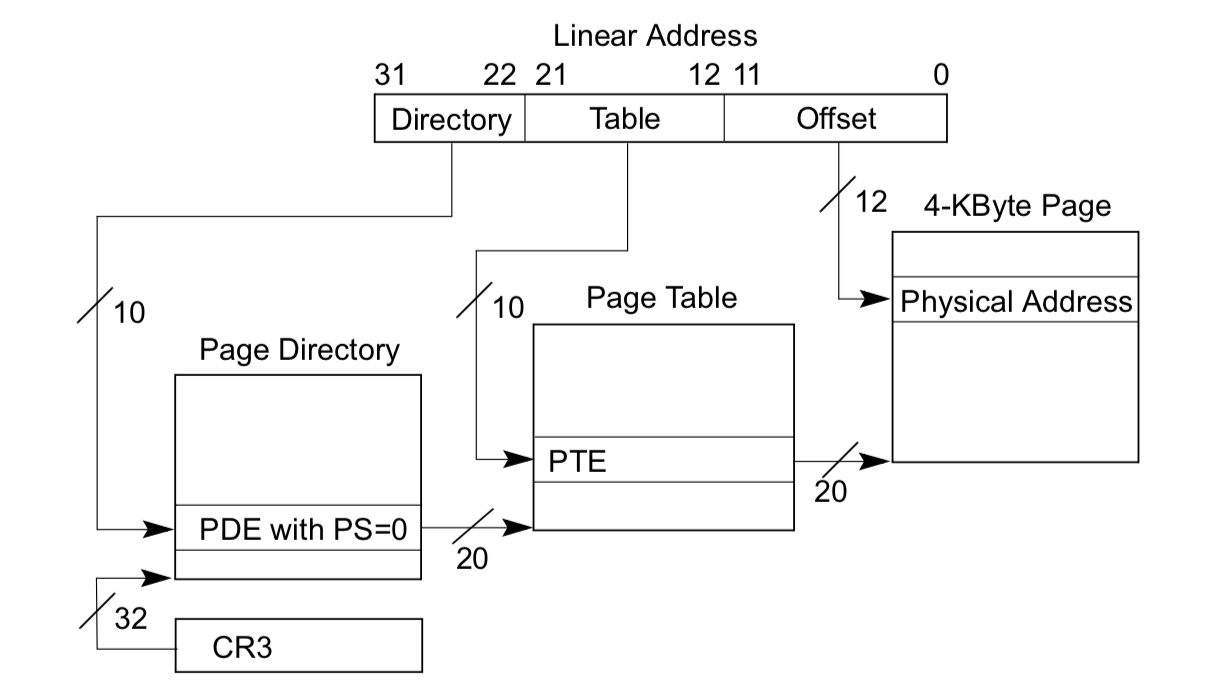
\includegraphics[width=10cm]{images/memory_page_table_32bits.png}
    \caption{\label{pic:memory_page_table_32bits} Table de pages utilisant 32 bits de l'adresse virtuelle dans une table à 3 niveaux \cite{intel64and}}.
\end{figure}

\begin{figure}
    \center
    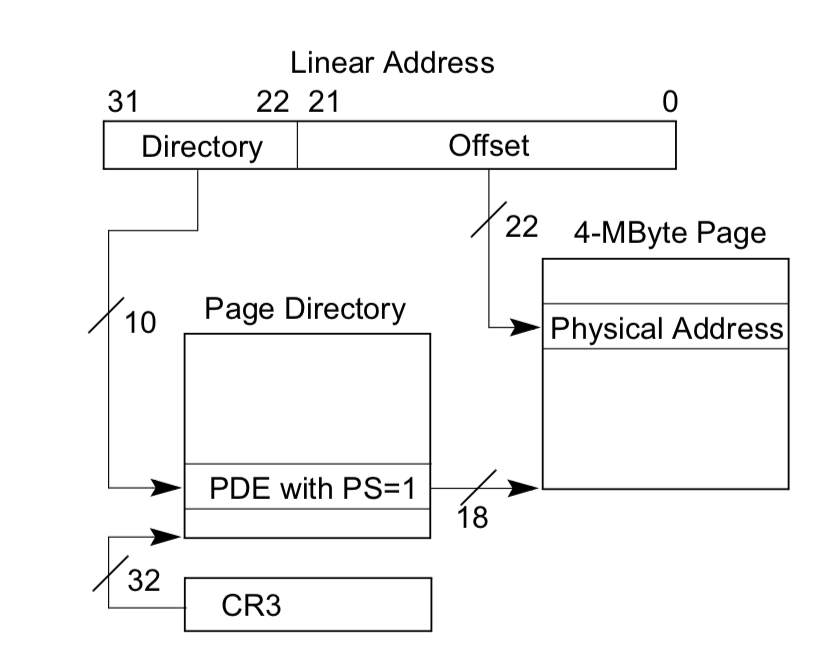
\includegraphics[width=10cm]{images/memory_page_table_32bits_large.png}
    \caption{\label{pic:memory_page_table_32bits_large} Table de pages pour des page large de 2 MiB\cite{intel64and}}.
\end{figure}


\begin{figure}
    \center
    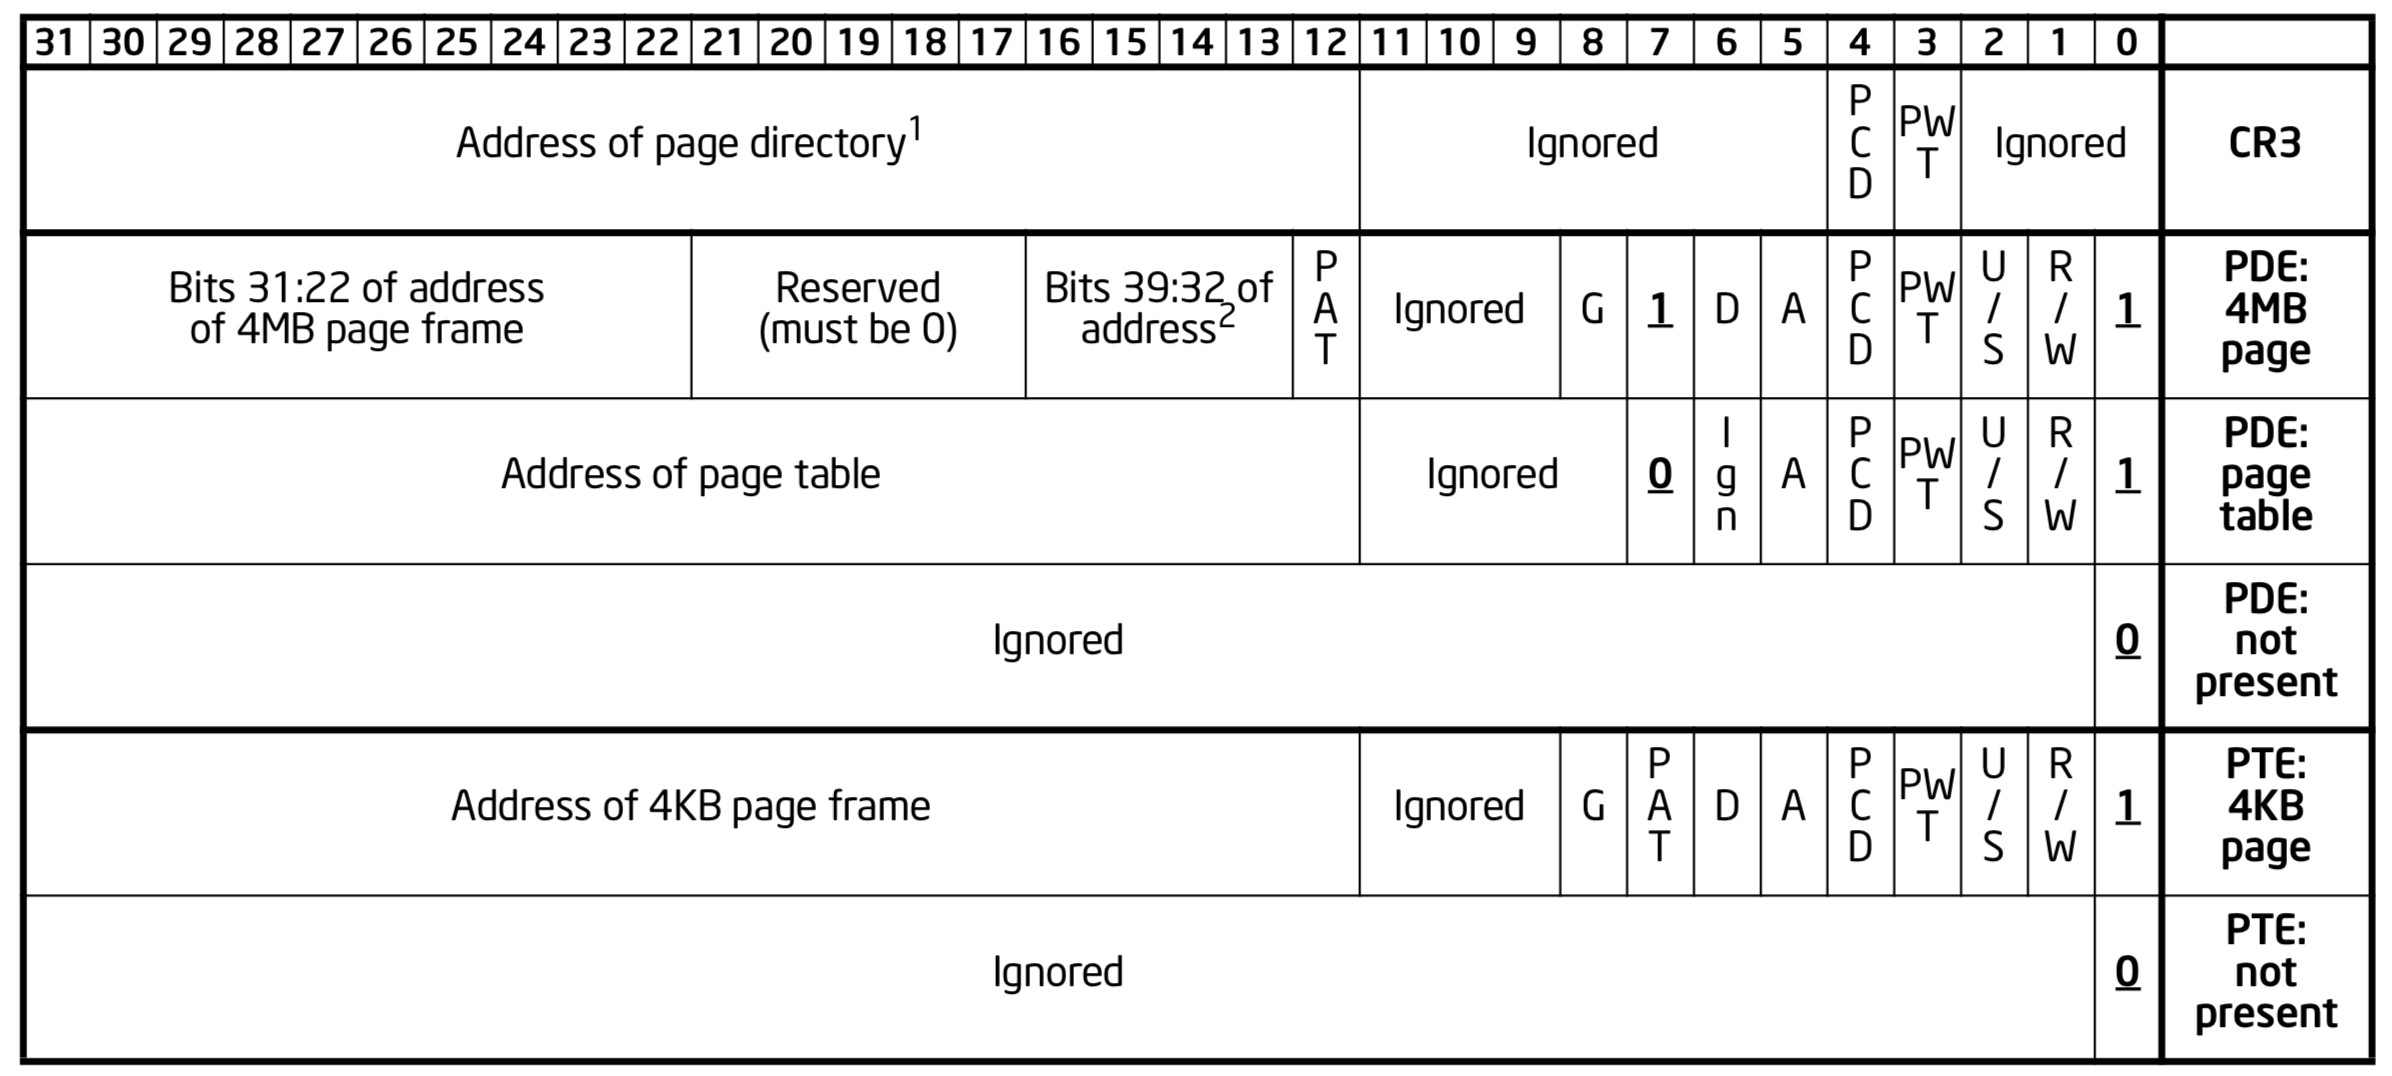
\includegraphics[width=10cm]{images/memory_page_table_entry_intel.png}
    \caption{\label{pic:memory_page_table_entry_intel} Structure d'une entrée dans la table de page \cite{intel64and}}.
\end{figure}



%\begin{figure}[p]
  %\centering
  %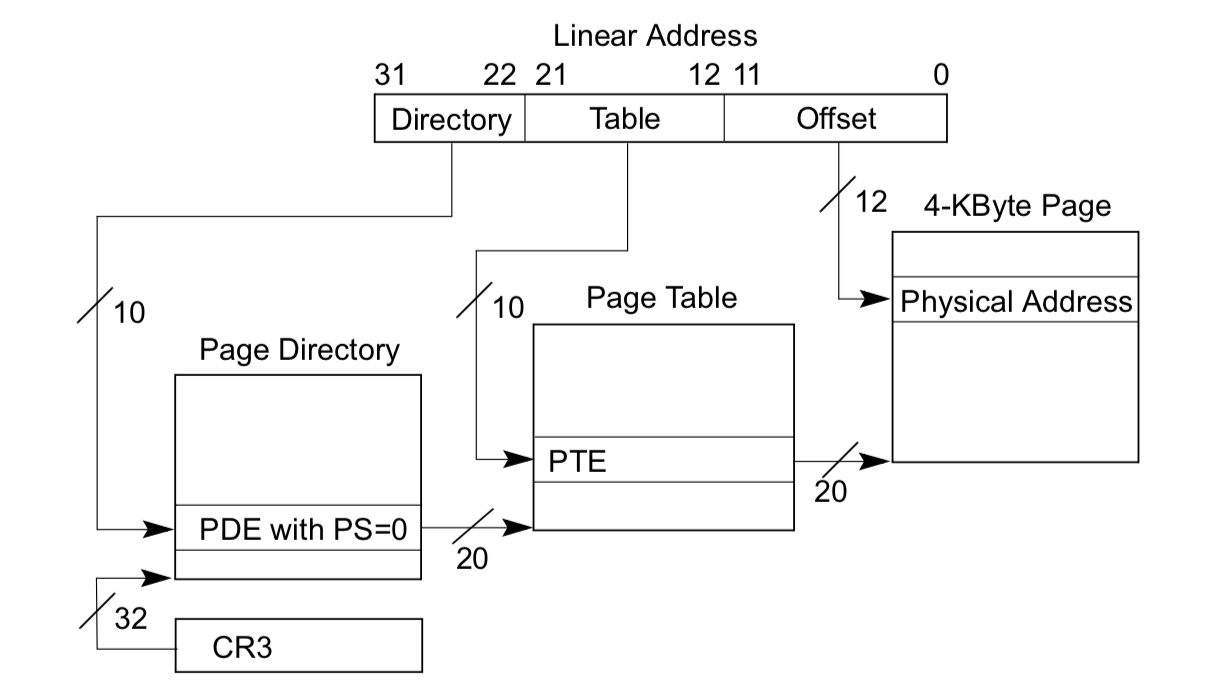
\includegraphics[width=0.2\textwidth]{images/memory_page_table_32bits.png}
  %\caption{Capt1.}
  %\label{fig:lab1}
  %\centering
  %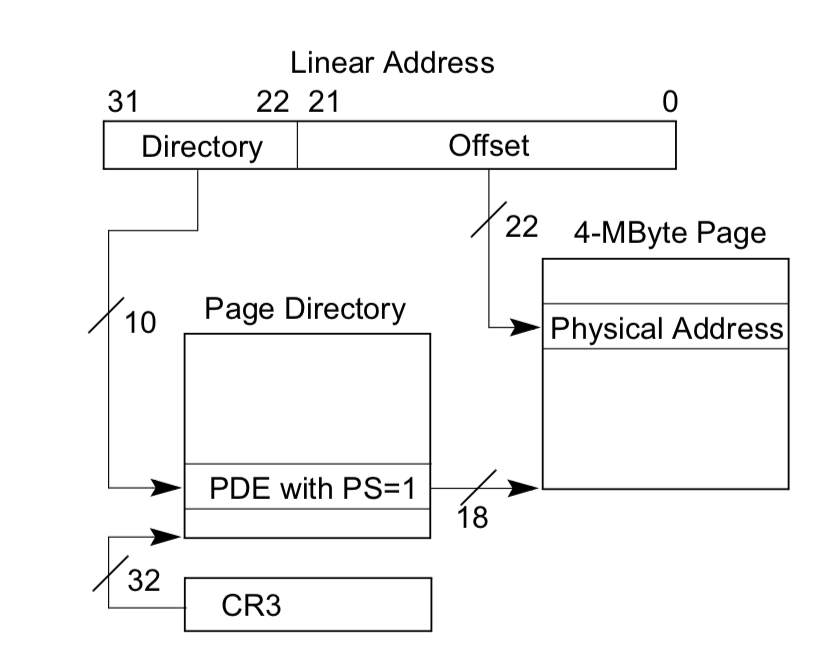
\includegraphics[width=0.2\textwidth]{images/memory_page_table_32bits_large.%png}
  %\caption{Capt2.}
  %\label{fig:lab2}
  %\centering
  %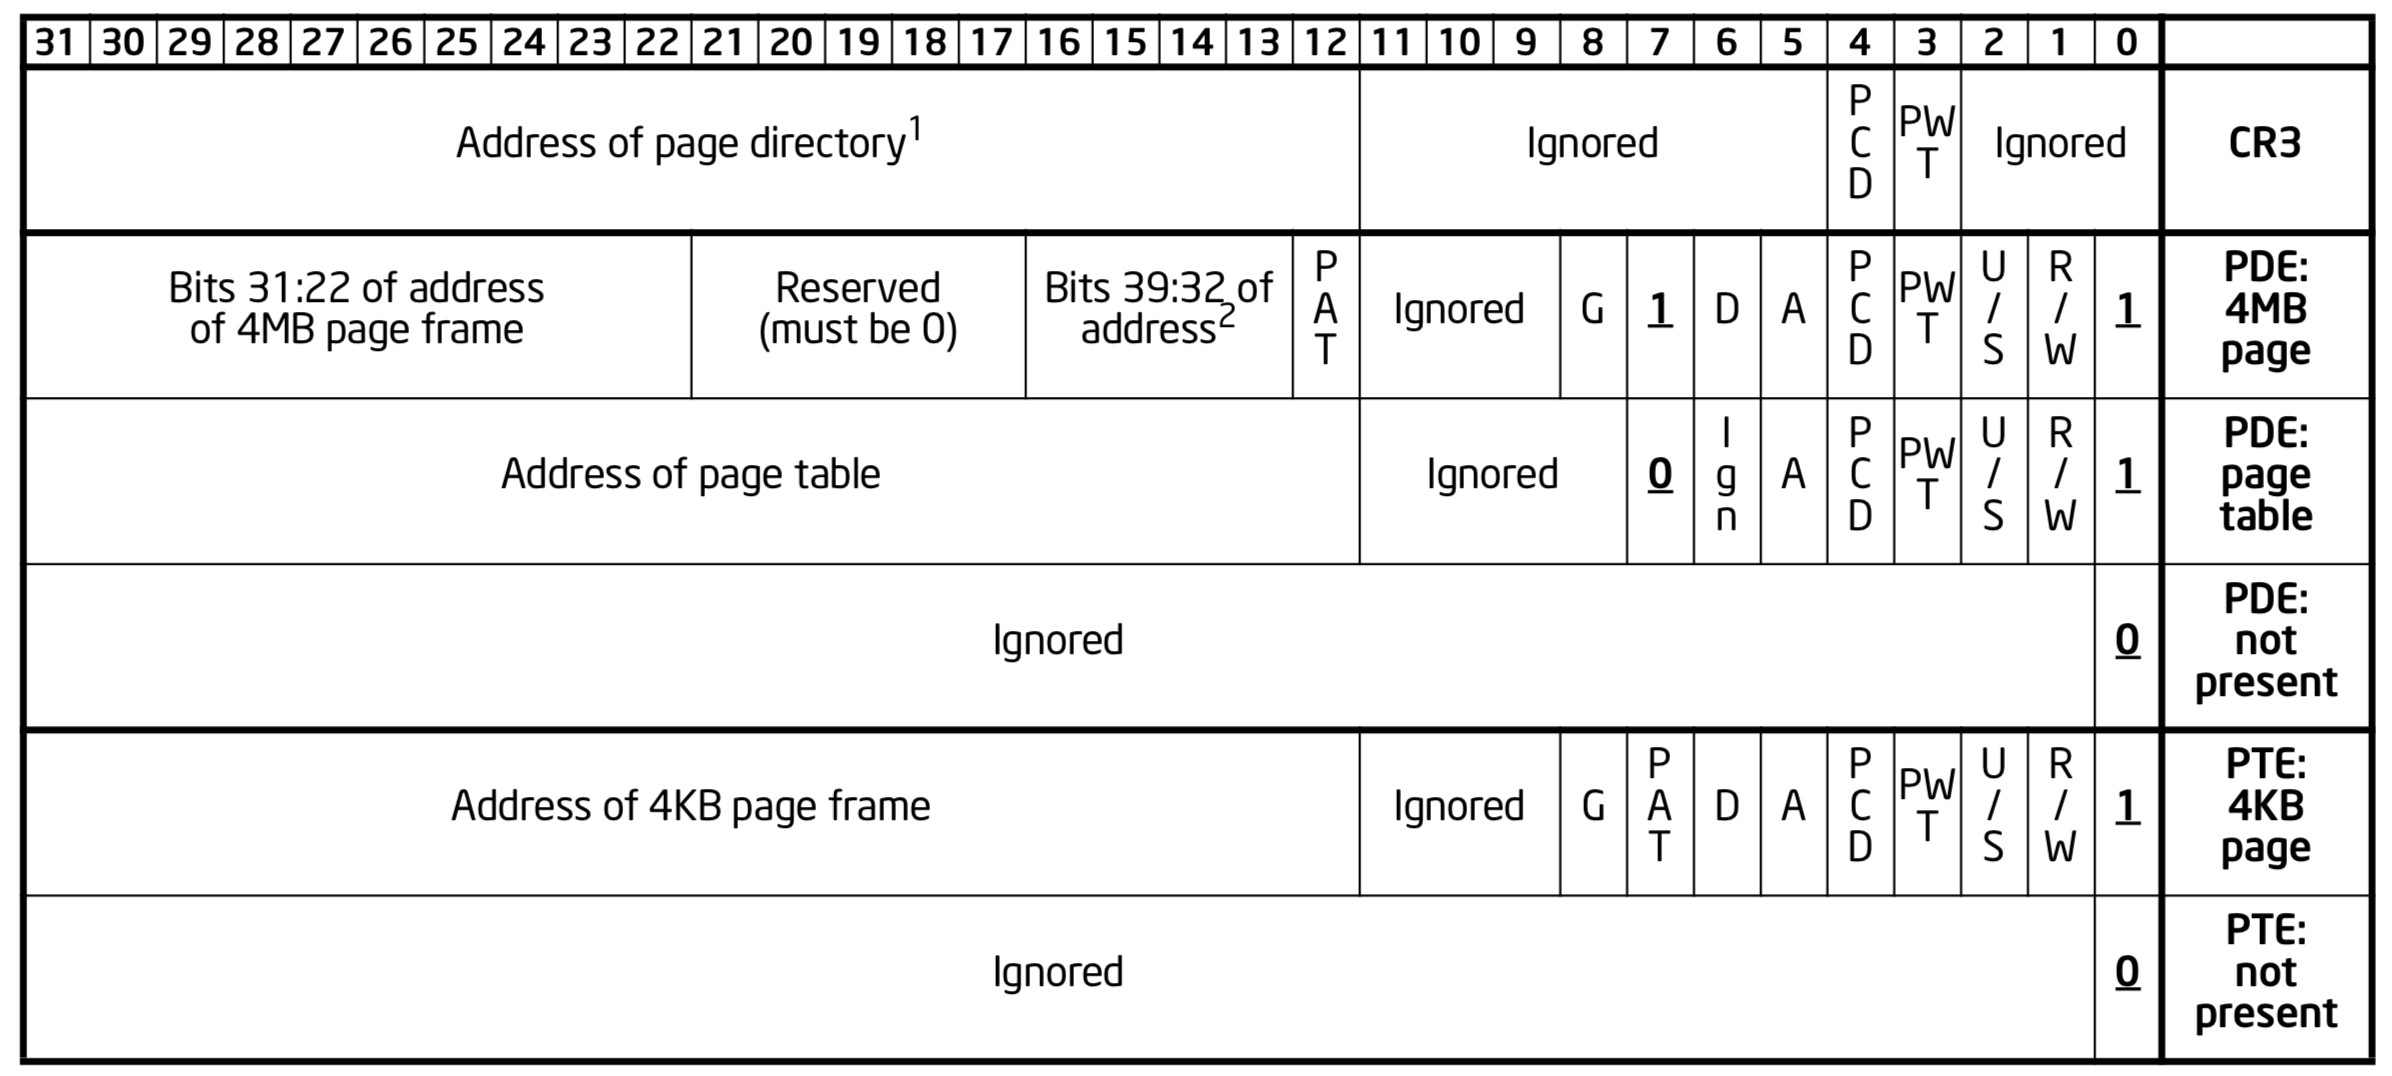
\includegraphics[width=0.2\textwidth]{images/memory_page_table_entry_intel.p%ng}
  %\caption{capt3.}
  %\label{fig:lab3}
%\end{figure}

\bibliographystyle{StyleThese}
\bibliography{These}

%\printnomenclature

\cleardoublepage
\begin{vcenterpage}
\noindent\rule[2pt]{\textwidth}{0.5pt}
\\
{\large\textbf{Résumé :}}
L'objectif de cette thèse est de fournir aux radiothérapeutes des outils de contourage automatique des structures à risque pour la planification de la radiothérapie des tumeurs cérébrales et de la région ORL.
\\
Nous utilisons pour cela un atlas anatomique, constitué d'une représentation de l'anatomie associée à une image de celle-ci. Le recalage de cet atlas permet de contourer automatiquement les organes du patient et ainsi obtenir un gain de temps considérable. Les contributions présentées se concentrent sur trois axes.
\\
Tout d'abord, nous souhaitons obtenir une méthode de recalage la plus indépendante possible du réglage de ses paramètres. Celui-ci, effectué par le médecin, se doit d'être minimal, tout en garantissant un résultat robuste. Nous proposons donc des méthodes de recalage permettant un meilleur contrôle de la transformation obtenue, en passant par des techniques de rejet d'appariements aberrants ou en utilisant des transformations localement affines.
\\
Le second axe est consacré à la prise en compte de structures dues à la tumeur. En effet, la présence de ces structures, absentes de l'atlas, perturbe le recalage de celui-ci. Nous proposons donc également des méthodes afin de contourer ces structures et de les prendre en compte dans le recalage.
\\
Enfin, nous présentons la construction d'un atlas ORL et son évaluation sur une base de patients. Nous montrons ici la faisabilité de l'utilisation d'un atlas de cette région, ainsi qu'une méthode simple afin d'évaluer les méthodes de recalage utilisées pour construire un atlas.
\\
L'ensemble de ces travaux a été implémenté dans le logiciel Imago de DOSIsoft, ceci ayant permis d'effectuer une validation en conditions cliniques.
\\
\\
{\large\textbf{Mots clés :}}
Segmentation par atlas, recalage non linéaire, radiothérapie, création d'atlas
\\
\noindent\rule[2pt]{\textwidth}{0.5pt}
\end{vcenterpage}

\begin{vcenterpage}
\noindent\rule[2pt]{\textwidth}{0.5pt}
\begin{center}
{\large\textbf{Design and Use of Numerical Anatomical Atlases for Radiotherapy\\}}
\end{center}
{\large\textbf{Abstract:}}
The main objective of this thesis is to provide radio-oncology specialists with automatic tools for delineating organs at risk of a patient undergoing a radiotherapy treatment of cerebral or head and neck tumors.
\\
To achieve this goal, we use an anatomical atlas, i.e. a representative anatomy associated to a clinical image representing it. The registration of this atlas allows to segment automatically the patient structures and to accelerate this process. Contributions in this method are presented on three axes.
\\
First, we want to obtain a registration method which is as independent as possible w.r.t. the setting of its parameters. This setting, done by the clinician, indeed needs to be minimal while guaranteeing a robust result. We therefore propose registration methods allowing to better control the obtained transformation, using outlier rejection techniques or locally affine transformations.
\\
The second axis is dedicated to the consideration of structures associated with the presence of the tumor. These structures, not present in the atlas, indeed lead to local errors in the atlas-based segmentation. We therefore propose methods to delineate these structures and take them into account in the registration.
\\
Finally, we present the construction of an anatomical atlas of the head and neck region and its evaluation on a database of patients. We show in this part the feasibility of the use of an atlas for this region, as well as a simple method to evaluate the registration methods used to build an atlas.
\\
All this research work has been implemented in a commercial software (Imago from DOSIsoft), allowing us to validate our results in clinical conditions.
\\
\\
{\large\textbf{Keywords:}}
Atlas-based Segmentation, non rigid registration, radiotherapy, atlas creation
\\
\noindent\rule[2pt]{\textwidth}{0.5pt}
\end{vcenterpage}

\end{document}
